\section*{Learning Objectives}

\begin{itemize}
\item Null space of a matrix and relation to linear independence
\item  Regression
\item Debugging, or finding and fixing errors in your code
\end{itemize}

\section*{Outcomes} 
\begin{itemize}
\item A new way to check for linear independence
\item A brief introduction to basis vectors
\item Practice with a linear algebra Super Power, Linear Regression
\item Practice with ``broadcasting''
\item Practice with plotting
\item Knowledge that you can use linear regression to fit nonlinear functions to ``curved data''  as long as the unknown coefficients enter in a linear manner
\end{itemize}

\vspace*{1cm}

\textbf{Either download Lab6 from our Canvas site or open up a Jupyter notebook so that you can enter code as we go. It is suggested that you have line numbering toggled on.}  

\newpage

We've covered most of the Julia coding that we need for ROB 101. This lab will focus on the null space of a matrix and linear regression. 

\section{Null Space of a Matrix}

The null space of a matrix can be used to find linear combinations of vectors that add up to zero. Specifically, consider a set of vectors $\{ v_1, v_2, \ldots, v_m\} \subset \real^n$ and form the $n \times m$ matrix 
$$A = \left[ v_1 ~ v_2 ~\cdots ~v_m\right].$$ 
From lecture, the \textbf{null space of $A$} is 
$${\rm null}(A):=\{x \in \real^m~| ~ A x = 0_{n \times 1}   \}. $$
If $x \in {\rm null}(A)$ and $x \neq 0_{m \times 1} $, then we have a set of non-zero coefficients such 
$$x_1 v_1 + x_2 v_2 + \ldots + x_m v_m = 0_{n \times 1} $$
which means the set of vectors is \textbf{linearly dependent}. On the other hand, if the null space of $A$ consists only of the zero vector, then the set of vectors is \textbf{linearly independent}.

\begin{rem} If you do not like denoting the coefficients in the linear combination by $x_i$, then we can use $\alpha_i$ instead and write 
$$A \cdot \alpha = 0_{n \times 1} \iff \alpha_1 v_1 + \alpha_2 v_2 + \ldots + \alpha_m v_m = 0_{n \times 1}.$$
\end{rem}

\begin{lstlisting}[language=Julia,style=mystyle]
# The nullspace command in Julia LinearAlgebra package
using LinearAlgebra

A = [1 2 3 4; 5 6 7 8; 9 10 11 12]
V = nullspace(A)
\end{lstlisting}
\textbf{Output} 
\begin{verbatim}
4×2 Matrix{Float64}:
  0.261535  -0.481248
 -0.707414   0.446727
  0.630224   0.550289
 -0.184345  -0.51576
\end{verbatim}

\begin{lstlisting}[language=Julia,style=mystyle]
v1 = V[:,1]
v2 = V[:,2]
@show A*v1 # needs to be zero for v1 to be in the null space
@show A*v2 # similar. 
\end{lstlisting}
\textbf{Output} 
\begin{verbatim}
A * v1 = [-1.1102230246251565e-16, 2.220446049250313e-16, 2.220446049250313e-15]
A * v2 = [0.0, -8.881784197001252e-16, -8.881784197001252e-16]

3-element Vector{Float64}:
  0.0
 -8.881784197001252e-16
 -8.881784197001252e-16
\end{verbatim}

We check that vectors in the null space tell us how to form linear combinations of the columns of $A$ that add up to zero. \\

\begin{lstlisting}[language=Julia,style=mystyle]
# Linear combination of the columns of A that adds up to zero
a1=V[1,1]
a2=V[2,1]
a3=V[3,1]
a4=V[4,1]
#
a1*A[:,1] + a2*A[:,2] + a3*A[:,3] + a4*A[:,4]
\end{lstlisting}
\textbf{Output} 
\begin{verbatim}
3-element Vector{Float64}:
 -1.1102230246251565e-16
  2.220446049250313e-16
  2.220446049250313e-15
\end{verbatim}

\begin{lstlisting}[language=Julia,style=mystyle]
# Linear combination of the columns of A that adds up to zero
a1=V[1,2]
a2=V[2,2]
a3=V[3,2]
a4=V[4,2]
#
a1*A[:,1] + a2*A[:,2] + a3*A[:,3] + a4*A[:,4]
\end{lstlisting}
\textbf{Output} 
\begin{verbatim}
3-element Vector{Float64}:
  0.0
 -8.881784197001252e-16
 -8.881784197001252e-16
\end{verbatim}

We also recall from lecture that the null space of a matrix is a subspace. Indeed, $v_i \nullspace(A) \iff A v_1 = 0_{n \times 1}$, and thus, if we consider a linear combination of vectors in the null space of $A$, and apply $A$ to it, we get the zero vector. Indeed, 
$$A \cdot(\alpha_1 v_1 + \alpha_2 v_2) = \alpha_1 A \cdot v_1 + \alpha_2 A \cdot v_2 = \alpha_1 0_{n \times 1} + \alpha_2 0_{n \times 1}  =  0_{n \times 1}.$$
So, if a null space is a subspace, why is the command \texttt{nullspace} only returning two vectors? \\

\begin{lstlisting}[language=Julia,style=mystyle]
# The nullspace command in Julia LinearAlgebra package
using LinearAlgebra

A = [1 2 3 4; 5 6 7 8; 9 10 11 12]
println("If a null space is a subspace, why is the command only returning two vectors?")
V = nullspace(A)
\end{lstlisting}
\textbf{Output} 
\begin{verbatim}
If a null space is a subspace, why is the command only returning two vectors?

4×2 Matrix{Float64}:
  0.261535  -0.481248
 -0.707414   0.446727
  0.630224   0.550289
 -0.184345  -0.51576
\end{verbatim}

The \texttt{nullspace} command in Julia is returning a ``basis'' for the subspace. When you are first reading this, we may not have covered the concept of basis vectors in lecture. Hence, we give a preview of the definition here.


\begin{tcolorbox}[title=\textbf{Preview of Basis Vectors}] We are delaying the formal study of basis vectors until Chapter~10 in our textbook. In the meantime, it helps to have an intuitive understanding:
\begin{itemize}
    \item A set of vectors $\{ v_1, v_2,  \ldots, v_m\} \subset V$ is a \textbf{basis for $V$} if
    \begin{enumerate}
    \renewcommand{\labelenumi}{(\alph{enumi})}
\setlength{\itemsep}{.2cm}
        \item $\{ v_1, v_2,  \ldots, v_m\}$ is linearly independent
        \item $x\in V \iff$ there exist coefficients $\alpha_1, \ldots, \alpha_m$ such that $x = \alpha_1 v_1  + \cdots + \alpha_m v_m$.
    \end{enumerate}
\item Personally, your instructor likes to think of a basis $\{ v_1, v_2,  \ldots, v_m\} \subset V$ in the following way:
\begin{enumerate}
    \renewcommand{\labelenumi}{(\alph{enumi})}
\setlength{\itemsep}{.2cm}
    \item  The set $\{ v_1, v_2,  \ldots, v_m\}$  is \textbf{big enough to generate $V$ by forming linear combinations}, and
    \item \textbf{small enough to be linearly independent}.
    \end{enumerate}
\end{itemize}
 
\end{tcolorbox}

\vspace*{.2cm}

\textbf{A Goldilocks interpretation of a basis for a subspace $V$}: \textcolor{red}{\bf a basis is a set of vectors that is not too big and not too small.} 
\begin{itemize}

    \item If every $x \in V$ can be expressed as a linear combination of elements of $\{ v_1, v_2,  \ldots, v_m\}$, then  $\{ v_1, v_2,  \ldots, v_m\}$ is \textbf{big enough} to ``generate'' all of $V$. 
        \item If the set  $\{ v_1, v_2,  \ldots, v_m\}$ is linearly independent, then it is \textbf{small enough} that you cannot discard elements without changing the number of linearly independent vectors.
        \item Hence, a basis is \textbf{``just right''} in terms of the quantity of vectors you need to build every vector in the subspace through the operation of forming linear combinations.
\end{itemize}

\vspace*{.2cm}

\begin{tcolorbox}[title=\textbf{Another Test for Linear Independence}] Consider a set of vectors in $\real^n$,
$$\left\{v_1=\begin{bmatrix} a_{11} \\ a_{21}\\ \vdots \\ a_{n1} \end{bmatrix},  v_2=\begin{bmatrix} a_{12} \\ a_{22}\\ \vdots \\ a_{n2} \end{bmatrix}, ...,  v_m=\begin{bmatrix} a_{1m} \\ a_{2m}\\ \vdots \\ a_{nm} \end{bmatrix} \right\},$$ 
and use them as the columns of a matrix that we call $A$,
\begin{equation}
\label{eq:MatrixFromLinearIndependence_proTipCC}    
A=\left[\begin{array}{cccc} a_{11}& a_{12}& \cdots & a_{1m} \\
 a_{21}& a_{22}& \cdots & a_{2m}  \\
 \vdots & \vdots&  \ddots & \vdots \\
 a_{n1}& a_{n2}& \cdots & a_{nm} 
 \end{array}\right].
 \end{equation}
 The following statements are equivalent:
 \begin{itemize}
     \item  The set of vectors $ \{v_1, v_2, \ldots, v_m \} $ is linearly independent.
     \item The null space of $A$ is the zero vector, that is, the only vector $x\in \real^m$ satisfying $Ax = 0_{n \times 1}$ is the vector $x = 0_{m \times 1}$
 \end{itemize}
\end{tcolorbox}

\vspace*{.2cm}

Determine if the set of vectors $\{v_1, v_2, v_3, v_4\}$ is linearly independent or not. 
\begin{lstlisting}[language=Julia,style=mystyle]
using Random
Random.seed!(2021)
v1=randn(5,1)
v2=randn(5,1)
v3=randn(5,1)
v4=randn(5,1)

# Place your code below
A = [v1 v2 v3 v4]
println("Note how Julia reports that there are no non-zero vectors satisfying Ax = 0")
V = nullspace(A)
\end{lstlisting}
\textbf{Output} 
\begin{verbatim}
Note how Julia reports that there are no non-zero vectors satisfying Ax = 0

4×0 Matrix{Float64}
\end{verbatim}

\vspace*{.2cm}

Julia reported an ``empty basis''... there are no non-zero vectors required to generate the null space of $A$.\\

 Determine if the set of vectors $\{v_1, v_2, ..., v_6\}$ is linearly independent or not. If they are linearly dependent, find a set of not all identically zero coefficients such that $\alpha_1 v_1 + \alpha_2 v_2 + \cdots + \alpha_6 v_6= 0$. In other words, find a non-trivial linear combination of the set of vectors that adds up to the zero vector.\\

\begin{lstlisting}[language=Julia,style=mystyle]
using Random
Random.seed!(2021)
v1=randn(4,1)
v2=randn(4,1)
v3=randn(4,1)
v4=randn(4,1)
v5=randn(4,1)
v6=randn(4,1)

# Place your code below
# Compute alpha = [alpha1; alpha2; ...; alpha6]
# such that alpha1*v1 + alpha2*v2 + ... + alpha6*v6 = 0
# your code here
A = [v1 v2 v3 v4 v5 v6]
V = nullspace(A)
\end{lstlisting}
\textbf{Output} 
\begin{verbatim}
6×2 Matrix{Float64}:
 -0.884195    0.175427
 -0.0530824   0.686466
 -0.254579    0.093228
 -0.274888   -0.461607
  0.158941   -0.150481
  0.223037    0.50356
\end{verbatim}

\vspace*{.2cm}

\begin{lstlisting}[language=Julia,style=mystyle]
# solution continued
alpha = sqrt(3)*V[:,1] + pi*V[:,2]
\end{lstlisting}
\textbf{Output} 
\begin{verbatim}
6-element Vector{Float64}:
 -0.9803501037910766
  2.064655155074321
 -0.14805907841326366
 -1.926298965466871
 -0.19745609676639247
  1.9682934386167301
\end{verbatim}

\vspace*{.2cm}

\begin{lstlisting}[language=Julia,style=mystyle]
A*alpha
\end{lstlisting}
\textbf{Output} 
\begin{verbatim}
4-element Vector{Float64}:
  4.996003610813204e-16
  0.0
 -8.881784197001252e-16
  0.0
\end{verbatim}

%\vspace*{.2cm}

\section{Linear Regression or Least Squares Fit to Data}
\label{sec:LinearRegression}

We seek to fit a function to data. For example, we have a scatter plot of data points and wish to approximate the points with a straight line or perhaps a polynomial. It is assumed that you have scanned Chapter 8 in our textbook (not the Lab Manual).\\

% \begin{figure}[htb]%
% 	\centering
% 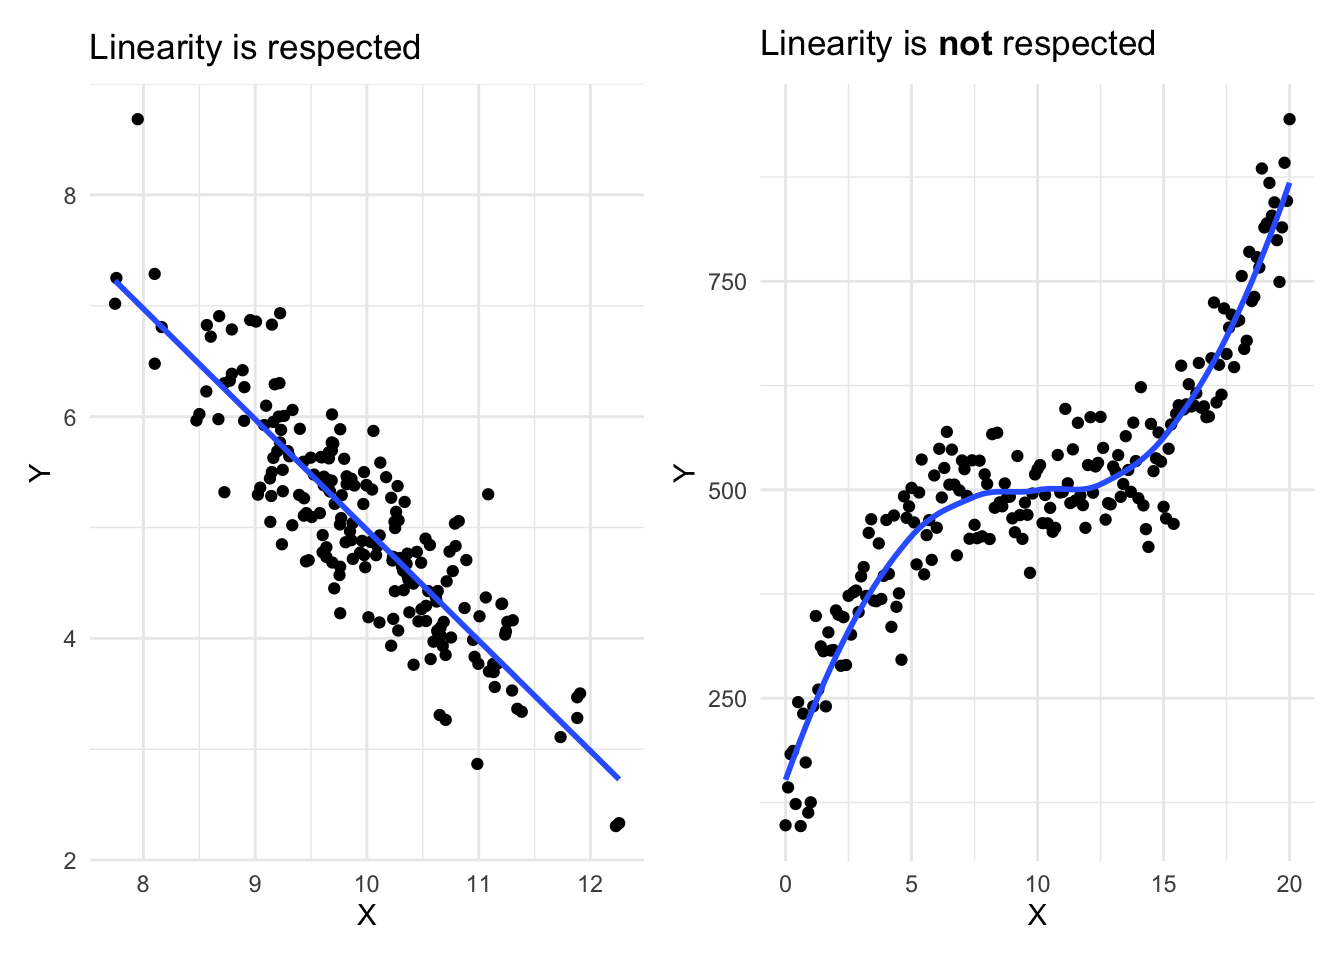
\includegraphics[width=0.6\columnwidth]{graphics/Chap06/Regression.png}
% \caption[]{From \url{https://www.r-bloggers.com/2021/10/multiple-linear-regression-made-simple/}. The first step is to plot your data and decide if you are fitting a line or something more complicated. As we will see, both can be accommodated via linear regression.}
%     \label{fig:Regression}
% \end{figure}

 The first step is to plot our data and decide if we are fitting a line or something more complicated. As we will see, both can be accommodated via linear regression.

\begin{lstlisting}[language=Julia,style=mystyle]
# Generate some points for line fitting
# Run me, don't change me. 
using Random
Random.seed!(2021)
NumPts = 100
m = 2
b = 1
x = -1 .+ 2*rand(NumPts,1)
y = m*x .+ b + 0.30*randn(NumPts, 1)

using Plots
scatter(x, y, legend=false)
\end{lstlisting}
\textbf{Output} 

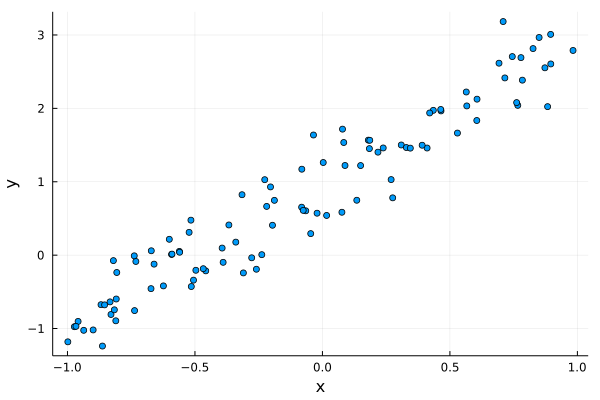
\includegraphics[width=0.6\columnwidth]{graphics/Chap06/LinearScatterPlot.png}

This looks appropriate for fitting a line. Hence, we assume a linear model ${y}=mx+b$. We set up the linear equations
$$y_i = b + m x_i  = \begin{bmatrix}  1 & x_i  \end{bmatrix} \begin{bmatrix} b \\ m \end{bmatrix},  ~~1 \le i \le N,$$ 
where $N$ is the number of data points (100 in our case), and write it out in matrix form
\begin{equation}
    \label{eq:FirstRegressionModel02}
\underbrace{\begin{bmatrix} y_1 \\ y_2 \\ \vdots \\y_N \end{bmatrix}}_{Y} = \underbrace{\left[\begin{array}{cc}
 1 &   x_1\\
  1 &     x_2  \\
  1 &     \vdots  \\
   1 &    x_N 
\end{array}  \right]}_{\Phi} \cdot  \underbrace{\begin{bmatrix} b \\ m \end{bmatrix}}_{\alpha},
\end{equation}
where $Y$ is the vector of $y$-data, $\Phi$ is called the \textbf{regressor matrix} and $\alpha$ is the vector of \textbf{unknown coefficients} that parameterize the  model.
\begin{lstlisting}[language=Julia,style=mystyle]
# Create the Y and the regressor matrix Phi
# Run me, don't change me.
Y = y
Phi = [ones(NumPts,1) x]
\end{lstlisting}
\textbf{Abridged Output} 
\begin{verbatim}
100×2 Matrix{Float64}:
 1.0  -0.188407
 1.0  -0.868452
 1.0  -0.203676
 1.0  -0.672369
 1.0   0.566187
 1.0  -0.731769
 .
 .
 .
 1.0   0.39111
 1.0  -0.0753372
 1.0   0.149722
 1.0  -0.816126
 1.0   0.420627
\end{verbatim}

\begin{tcolorbox}[title=\textbf{\large Least Squares Fit to Data also called Linear Regression}]

 From our textbook, if the columns of $\Phi$ are linearly independent, or equivalently, $\Phi^\top \Phi$ is invertible, then the following are equivalent 
  \begin{equation}
    \label{eq:ThmLeastSqaredErrorSolution2}
  \alpha^\ast = \left( \Phi^\top \Phi \right)^{-1}\Phi^\top Y  \iff  \alpha^\ast = \argmin_{\alpha} ||Y-\Phi \alpha ||^2 \iff \left( \Phi^\top \Phi \right) \alpha^\ast = \Phi^\top Y.
\end{equation}
  
  \end{tcolorbox}


\begin{lstlisting}[language=Julia,style=mystyle]
# OK for small problems, such as here, with two unknowns
A=Phi'*Phi
b=Phi'*Y
alpha = inv(A)*b
\end{lstlisting}
\textbf{Output} 
\begin{verbatim}
2×1 Matrix{Float64}:
 0.9472834926740609
 1.9393293464390031
\end{verbatim}


\begin{lstlisting}[language=Julia,style=mystyle]
scatter(x, y, legend=false)
y_hat = Phi * alpha
scatter!(x, y_hat)
titre="Regressed Line in Brown"
plot!(xlabel = "x", ylabel = "y", title=titre)
\end{lstlisting}
\textbf{Output} 

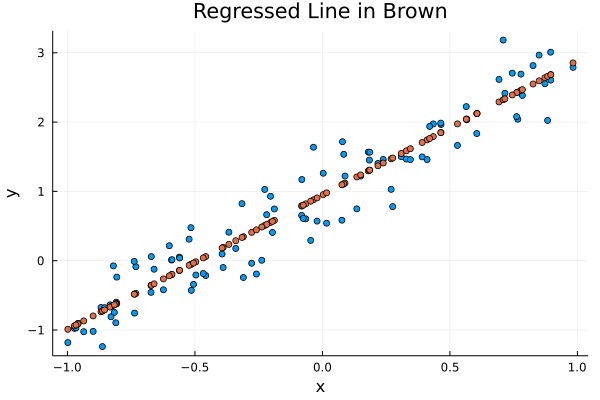
\includegraphics[width=0.6\columnwidth]{graphics/Chap06/LinearScatterPlotOverlay.png}

\begin{lstlisting}[language=Julia,style=mystyle]
# Generate some data for polynomial curve fitting
# Run me, don't change me.
#
using Random
Random.seed!(123456789)
NumPts = 100
x = -1 .+ 3*rand(NumPts,1)
a0 = 3
a1 = 6
a2 = 4
a3 = 6
a4 = -11
a5 = 2
a6 = -.2
# note the sin(2x) term
y = a6*x.^6 + a5*x.^5 + a4*x.^4 + a3*x.^3 + 
       a2*x.^2 .+ a1*sin.(2*x) .+ a0 + 1.50*randn(NumPts, 1)

using Plots
scatter(x,y,legend=false)
#png("PolyScatterPlot")
\end{lstlisting}
\textbf{Output} 

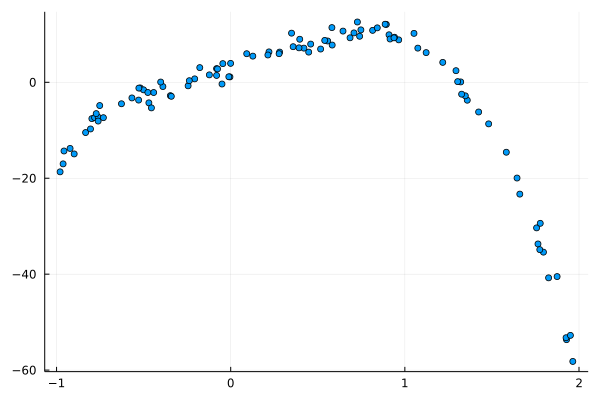
\includegraphics[width=0.7\columnwidth]{graphics/Chap06/PolyScatterPlot.png}



\begin{tcolorbox}[sharp corners, colback=green!30, colframe=green!80!blue, title=\textbf{\Large Large Scale Least Squares via the LU Factorization}]
 From our textbook,  if the columns of $\Phi$ are linearly independent, or equivalently, $\Phi^\top \Phi$ is invertible, we know the following are equivalent 
  \begin{equation}
    \label{eq:ThmLeastSqaredErrorSolution2secondTime}
  \alpha^\ast = \left( \Phi^\top \Phi \right)^{-1}\Phi^\top Y  \iff  \alpha^\ast = \argmin_{\alpha} ||Y-\Phi \alpha ||^2 \iff \left( \Phi^\top \Phi \right) \alpha^\ast = \Phi^\top Y.
\end{equation}
The suggested ``pipeline'' for  computing a least squared error solution to $ \left( \Phi^\top \Phi \right) \alpha^\ast = \Phi^\top Y$ is 
\begin{itemize}
    \item factor $P \cdot \left( \Phi^\top \Phi \right)  =: L \cdot U$, that is, do the LU Factorization of $\Phi^\top \cdot \Phi$,
    \item compute $\overline{b}:= P \cdot \Phi^\top Y$, and then 
    \item solve $L y = \overline{b}$ via forward substitution, and
    \item solve $U \alpha^\ast =y$ via backward substitution.
\end{itemize}
\end{tcolorbox}

\begin{lstlisting}[language=Julia,style=mystyle]
# Run me, don't change me. I am providing some nice functions for you.
# Forward and Back substitution functions from HW04

# This is a back substitution function.  It solves for x in an equation Ux = b, 
# where U is upper triangular. The function assumes U and b are the correct 
# sizes. You can add error checking, if you wish.
function backwardsub(U, b)
    # Check if U is non-signular
    min_diagU = minimum(abs.(diag(U)))
    if min_diagU <  1E-10
        return false
    end
    n = length(b)
    x = Vector{Float64}(undef, n) 
    x[n] = b[n]/U[n,n]
    for i in n-1:-1:1
        x[i]=(b[i]- (U[i,(i+1):n])' *x[(i+1):n] )./U[i,i]
    end
    return x
end
# This is a forward substitution function. It solves for x in an equation Lx = b, 
# where L is lower triangular. # The function assumes L and b are the correct 
# sizes. You can add error checking, if you wish.
function forwardsub(L, b)
     # Check if L is non-signular
    min_diagL = minimum(abs.(diag(L)))
    if min_diagL <  1E-10
        return false
    end
    n = length(b)
    x = Vector{Float64}(undef, n); 
    x[1] = b[1]/L[1,1] 
    for i = 2:n 
        x[i]=(b[i]- (L[i,1:i-1])' *x[1:i-1] )./L[i,i] 
    end
    return x
end
\end{lstlisting}
\textbf{Output} 
\begin{verbatim}
forwardsub (generic function with 1 method)
\end{verbatim}

\begin{lstlisting}[language=Julia,style=mystyle]
# Create the Y and the regressor matrix Phi
# Run me, don't change me.
Y = y
Phi = [ones(NumPts,1) x x.^2 x.^3 x.^4]
\end{lstlisting}
\textbf{Abridged Output} 
\begin{verbatim}
100×5 Matrix{Float64}:
 1.0   0.0919935   0.0084628    0.000778522   7.16189e-5
 1.0   0.90899     0.826264     0.751066      0.682712
 1.0   1.12227     1.25948      1.41347       1.58629
 1.0   1.58257     2.50452      3.96357       6.27261
 1.0   0.74038     0.548163     0.405849      0.300483
 1.0  -0.797207    0.63554     -0.506657      0.403911
 1.0  -0.206817    0.0427734   -0.00884629    0.00182957
 1.0  -0.177557    0.0315266   -0.00559777    0.000993924
 1.0   0.815018    0.664255     0.54138       0.441234
.
.
.
 1.0  -0.402096    0.161681    -0.0650113     0.0261408
 1.0   0.396441    0.157166     0.0623069     0.024701
 1.0  -0.0500005   0.00250005  -0.000125003   6.25023e-6
 1.0   0.685263    0.469585     0.321789      0.22051
 1.0  -0.898753    0.807756    -0.725973      0.65247
 1.0  -0.805068    0.648134    -0.521792      0.420078
\end{verbatim}


\begin{lstlisting}[language=Julia,style=mystyle]
# Find alpha by solving Phi' * Y= Phi' * Phi*alpha (Ax = b) using LU decomposition
using LinearAlgebra
F = lu(Phi' * Phi)
L = F.L
U = F.U
P = F.P
#
# Phi' * Y = Phi' * Phi * alpha
# after LU Factorization of Phi'*Phi, we have
# P *  Phi' * Y  = L * U * alpha
# 
y_alpha = forwardsub(L, P*Phi'*Y)
alpha = backwardsub(U, y_alpha)
\end{lstlisting}
\textbf{Output} 
\begin{verbatim}
5-element Vector{Float64}:
  3.71155035678547
 11.770104292873295
 -2.1786034505443537
  0.488282866753122
 -5.371244500774466
\end{verbatim}

\begin{lstlisting}[language=Julia,style=mystyle]
scatter(x, y, legend=false)
y_hat = Phi * alpha
scatter!(x, y_hat)
titre="Regressed Polynomial in Brown"
plot!(xlabel = "x", ylabel = "y", title=titre)
\end{lstlisting}
\textbf{Output} 


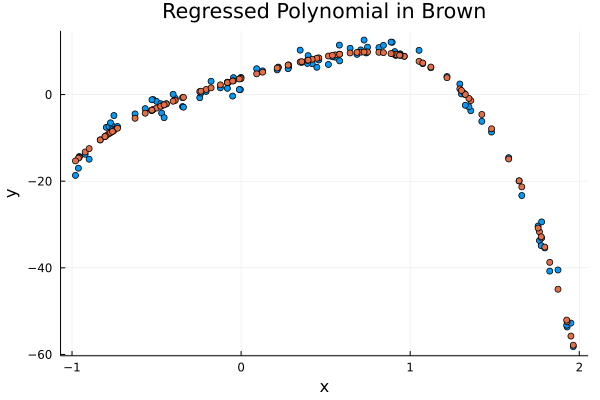
\includegraphics[width=0.7\columnwidth]{graphics/Chap06/PolyScatterPlotOverlay.png}

\section{Debugging}

Let's build a function \texttt{function LeastSquares\_Solve(Phi, Y)} that takes in a regressor matrix and a set of measurements, and returns the optimal parameters and data related to the quality of the fit. Because least squares fitting relies on solving $Ax=b$ when $A$ is square and invertible, we'll begin by building a function to compute exact solutions to square systems of linear equations. Moreover, we will build the function step-by-step and check for bugs as we go.\\
%%\label{sec:LinearRegression}

We start with baby steps. We only test for $A$ being square.
\begin{lstlisting}[language=Julia,style=mystyle]
# Function for solving Ax=b using LU decomposition
function Exact_Solve(A,b)
    nRows, nCols = size(A) 
    # We'll check for A not square. We assume A is a matrix.
    if ( nRows !== nCols)
         println("System of equations not properly formed")
        return x = NaN
    end
    xDummy= [1;2.0]
    return xDummy
end

A=[1 2; 3 4; 5 6]
b=[8; 9.0]
xAns = Exact_Solve(A,b)
\end{lstlisting}
\textbf{Output} 
\begin{verbatim}
System of equations not properly formed
NaN
\end{verbatim}
Next we add in a check that $b$ has the same number of rows as $A$. The command \texttt{||} ``double-pipes'' serves as the \texttt{logical or} command. We test it on good data and bad data. 

\begin{lstlisting}[language=Julia,style=mystyle]
# Function for solving Ax=b using LU decomposition
function Exact_Solve(A,b)
    nRows, nCols = size(A) 
    # We'll check for A not square. We assume A is a matrix.
    if ( nRows !== nCols)||(length(b) !== nRows)
         println("System of equations not properly formed")
        return x = NaN
    end
    xDummy= [1;2.0]
    return xDummy
end

A=[1 2; 3 4]
b=[8; 9.0; 11]
@show xAns = Exact_Solve(A,b)
b=[11, 13]
@show xAns = Exact_Solve(A,b);
\end{lstlisting}
\textbf{Output} 
\begin{verbatim}
System of equations not properly formed
xAns = Exact_Solve(A, b) = NaN
xAns = Exact_Solve(A, b) = [1.0, 2.0]
\end{verbatim}

Next we add in a solver via our beloved LU pipeline. We also check that the result is a valid solution of the equations.


\begin{lstlisting}[language=Julia,style=mystyle]
# Function for solving Ax=b using LU decomposition
function Exact_Solve(A,b)
    nRows, nCols = size(A) 
    # We'll check for A not square. We assume A is a matrix.
    if ( nRows !== nCols)||(length(b) !== nRows)
         println("System of equations not properly formed")
        return x = NaN
    end
    F=lu(A)
    y=forwardsub(F.L,F.P*b)
    x=backwardsub(F.U, y)
    return x
end

A=[1 2; 3 4]
b=[8; 9.0; 11]
@show xAns = Exact_Solve(A,b)
b=[11, 13]
@show xAns = Exact_Solve(A,b);
norm(A*xAns-b)
\end{lstlisting}
\textbf{Output} 
\begin{verbatim}
System of equations not properly formed
xAns = Exact_Solve(A, b) = NaN
xAns = Exact_Solve(A, b) = [-9.0, 10.0]

0.0
\end{verbatim}
We now add a tolerance and check for $A$ being singular. If $A$ is singular, we return \texttt{x=NaN}; otherwise, we implement the LU pipeline. We are very proud of our function!

\begin{lstlisting}[language=Julia,style=mystyle]
# Function for solving Ax=b using LU decomposition
function Exact_Solve(A,b,aTol=1e-10)
    nRows, nCols = size(A)
    if (length(b) !== nRows)||( nRows !== nCols)
         println("System of equations not properly formed")
        return x=NaN
    end
    F=lu(A)
    if minimum(abs.(diag(F.U))) < aTol
        println("diagU has numbers that are nearly zero")
        return x=NaN
    else
        y=forwardsub(F.L,F.P*b)
        x=backwardsub(F.U, y)
        return x 
    end
end

A=[1 1; 0 1e-14]
b=[8; 9.0]
@show xAns = Exact_Solve(A,b)
#
A=[1 1; 3 4]
b=[11, 13]
@show xAns = Exact_Solve(A,b)
norm(A*xAns-b)
\end{lstlisting}
\textbf{Output} 
\begin{verbatim}
diagU has numbers that are nearly zero
xAns = Exact_Solve(A, b) = NaN
xAns = Exact_Solve(A, b) = [31.00000000000001, -20.000000000000007]

3.552713678800501e-15
\end{verbatim}

Now we do a real life-size check! 

\begin{lstlisting}[language=Julia,style=mystyle]
using Random
A = randn(1000,1000)
b=randn(1000,1)
xAns = Exact_Solve(A,b);
norm(A*xAns-b)
\end{lstlisting}
\textbf{Output} 
\begin{verbatim}
2.643871993979311e-11
\end{verbatim}

And it looks great! So next, we develop a least squares solver. We use the fact that \texttt{alphaStar} satisfies
$$ \Phi^\top Y = \Phi^\top \cdot \Phi \alpha^\ast \iff \Phi^\top \cdot \Phi \alpha^\ast = \Phi^\top Y $$
and thus \texttt{alphaStar} should be the exact solution to $Ax=b$, for 
$$A \longleftrightarrow\Phi^\top \cdot \Phi , b\longleftrightarrow \Phi^\top Y, x \longleftrightarrow \alpha^\ast. $$


\begin{lstlisting}[language=Julia,style=mystyle]
# Function for fitting data with Least Squares
function LeastSquares_Solve(Phi, Y)
    alphaStar = Exact_Solve(Phi'*Phi, Phi'*Y) # Phi'*Y = Phi'*Phi * alpha
    # Return some extra quantities
    Yhat = Phi*alphaStar
    Error = Y-Yhat
    SqError = Error'*Error
    RootMeanSqError = sqrt(SqError/length(Y))
    return alphaStar, Yhat, RootMeanSqError
end
\end{lstlisting}
\textbf{Output} 
\begin{verbatim}
LeastSquares_Solve (generic function with 1 method)
\end{verbatim}

Now we run a real test!

\begin{lstlisting}[language=Julia,style=mystyle]
# Generate some data for polynomial curve fitting
# Run me, don't change me.
#
using Random
Random.seed!(123456789)
NumPts = 100
x = -1 .+ 2*rand(NumPts,1)
a0 = 3
a1 = 6
a2 = 4
a3 = 5
a4 = -5
y = a4*x.^4 + a3*x.^3 + a2*x.^2 .+ a1*x.^1 .+ a0 + 0.50*randn(NumPts, 1)

using Plots
scatter(x,y,legend=false, label="Y")

# Create the Y and the regressor matrix Phi
Y = y
Phi = [ones(NumPts,1) x x.^2 x.^3] # Fitting a cubic to a quartic

alphaStar, Yhat, RootMeanSqError = LeastSquares_Solve(Phi, Y)

println("The mean squared error is ", RootMeanSqError)

p1 = scatter!(x, Yhat, label="Y_hat")
png(p1, "LinearRegressionFit") 
display(p1)
\end{lstlisting}
\textbf{Output} 
\begin{verbatim}
The mean squared error is [0.6185570543212526]
\end{verbatim}



\begin{figure}[htb]%
	\centering
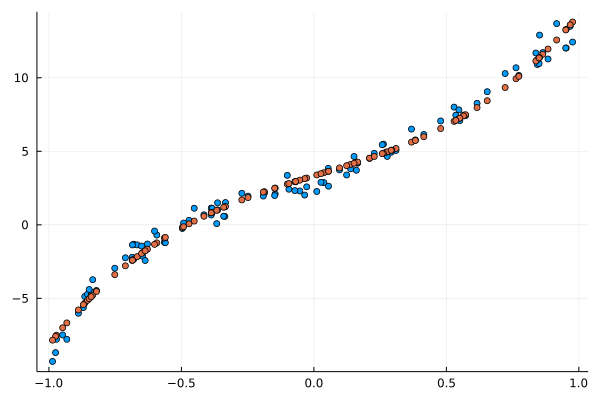
\includegraphics[width=0.7\columnwidth]{graphics/Chap06/Chap06LinearRegressionFit.png}
\caption[]{The blue dots are data while the orange dots are the fit to the data.}
    \label{fig:RegressionDebugging}
\end{figure}

\begin{tcolorbox}[title={\bf \Large Secret to Building Functions is to Check Them While Building Them}]

\textbf{Remarks:}
\begin{itemize}
    \item We broke our goal into two pieces, one solving an exact system of equations and one solving a least squares problem. 
    \item We included error checking as we went along and tested each piece.
    \item By the time we got to the end, the function that was new to us, one that solves a least squares problem, was a trivial extension of something familiar to us, solving a square system of equations with an invertible matrix.
    \item \textcolor{red}{\bf \Large You can do this too, even in HW problems:}
    \begin{itemize}
        \item Even when we say to place your code HERE, that code can include calls to other functions that you place in the same cell.
        \item {\bf \Large Really? Yes. Build a function called \texttt{LeastSquares\_Solve(Phi, Y)} that returns \texttt{alphaStar}}
    \end{itemize}
\end{itemize}
    
\end{tcolorbox}



\begin{lstlisting}[language=Julia,style=mystyle]
# Function for fitting data with Least Squares
function LeastSquares_Solve(Phi, Y)
    ### BEGIN SOLUTION

    ### END SOLUTION
    return alphaStar
end
\end{lstlisting}
\textbf{Output} 
\begin{verbatim}
LeastSquares_Solve (generic function with 1 method)
\end{verbatim}

\begin{lstlisting}[language=Julia,style=mystyle]
# Function for solving Ax=b using LU decomposition
function Exact_Solve(A,b,aTol=1e-10)
    nRows, nCols = size(A)
    if (length(b) !== nRows)||( nRows !== nCols)
         println("System of equations not properly formed")
        return x=NaN
    end
    F=lu(A,check=false)
    display(F)
    #indicesDiagUsmall=findall(x->x<aTol, abs.(diag(F.U)))
    if minimum(abs.(diag(F.U))) < aTol
        println("diagU has numbers that are nearly zero")
        return x=NaN 
    else
        y=forwardsub(F.L,F.P*b)
        x=backwardsub(F.U, y)
        return x 
    end
end


# Function for fitting data with Least Squares
function LeastSquares_Solve(Phi, Y)
    ### BEGIN SOLUTION
    alphaStar = Exact_Solve(Phi'*Phi, Phi'*Y) # Phi'*Y = Phi'*Phi * alpha
    ### END SOLUTION    
   return alphaStar
end
\end{lstlisting}
\textbf{Output} 
\begin{verbatim}
LeastSquares_Solve (generic function with 1 method)
\end{verbatim}

% \begin{lstlisting}[language=Julia,style=mystyle]

% \end{lstlisting}
% \textbf{Output} 
% \begin{verbatim}

% \end{verbatim}

% \begin{lstlisting}[language=Julia,style=mystyle]

% \end{lstlisting}
% \textbf{Output} 
% \begin{verbatim}

% \end{verbatim}

% \begin{lstlisting}[language=Julia,style=mystyle]

% \end{lstlisting}
% \textbf{Output} 
% \begin{verbatim}

% \end{verbatim}


\section{(Optional Read) Fitting a Surface to Data}

\begin{center}
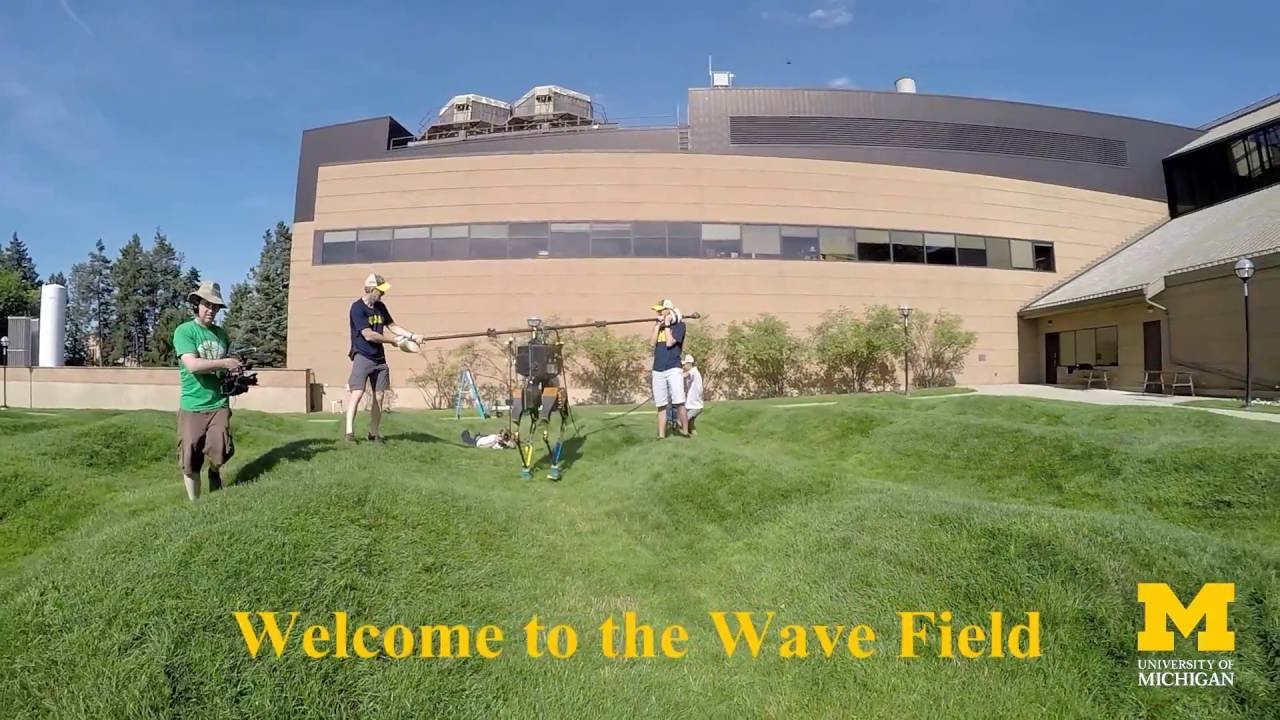
\includegraphics[width=0.8\columnwidth]{graphics/Chap06/WaveFieldMarlo.jpg}
\end{center}

We'll show that fitting a surface to data is the same as fitting a curve to data. Here, we'll continue using monomials as our basis functions. In Project 2, you will use radial basis functions, a better basis for surfaces with lots of curvature.\\


\begin{lstlisting}[language=Julia,style=mystyle]
# run me, don't change me
#
println("Be patient. It takes time to load the Distributions package.")
using Distributions
using Plots
using Pkg
Pkg.add("PyPlot")
\end{lstlisting}
\textbf{Output} 
\begin{verbatim}
Be patient. It takes time to load the Distributions package.

 Info: Precompiling Plots [91a5bcdd-55d7-5caf-9e0b-520d859cae80]
 @ Base loading.jl:1317
\end{verbatim}


\begin{lstlisting}[language=Julia,style=mystyle]
# Attempting to make the Wavefield!
z(x,y) = 0.2*sin(pi*x/2) - 0.2*cos(pi*y/3) + rand(Uniform(-0.03,0.03))

N = 100
Nsq = N^2
X = zeros(Nsq, 1)
Y = zeros(Nsq, 1)
Z = zeros(Nsq, 1)
for i = 1:N
    for j = 1:N
        X[(i-1)*N+j] = 10.0*i/N
        Y[(i-1)*N+j] = 10.0*j/N
        Z[(i-1)*N+j] = z(X[(i-1)*N+j], Y[(i-1)*N+j])
    end
end
scatter(X, Y, Z, marker_z=Z, legend=false, color = :greens, colorbar=true, camera=(-60, 60))
#png("WaveFieldData")
\end{lstlisting}
\textbf{Output} 
\begin{verbatim}
 Info: Precompiling GR_jll [d2c73de3-f751-5644-a686-071e5b155ba9]
 @ Base loading.jl:1317
 Warning: Module Cairo_jll with build ID 23135458039207652 is missing from the cache.
 This may mean Cairo_jll [83423d85-b0ee-5818-9007-b63ccbeb887a] does not support 
precompilation but is imported by a module that does.
 @ Base loading.jl:1008
 Info: Skipping precompilation since __precompile__(false). 
 Importing GR_jll [d2c73de3-f751-5644-a686-071e5b155ba9].
 @ Base loading.jl:1025
 Info: Precompiling Qt5Base_jll [ea2cea3b-5b76-57ae-a6ef-0a8af62496e1]
@ Base loading.jl:1317
 Warning: Module Glib_jll with build ID 23135459152168067 is missing from the cache.
 This may mean Glib_jll [7746bdde-850d-59dc-9ae8-88ece973131d] does not support 
precompilation but is imported by a module that does.
 @ Base loading.jl:1008
Info: Skipping precompilation since __precompile__(false). 
Importing Qt5Base_jll [ea2cea3b-5b76-57ae-a6ef-0a8af62496e1].
 @ Base loading.jl:1025
 Warning: camera: -60° not in [0°, 90°]
 @ Plots /opt/julia/packages/Plots/PomtQ/src/backends/gr.jl:1438
\end{verbatim}

\vspace*{.2cm}

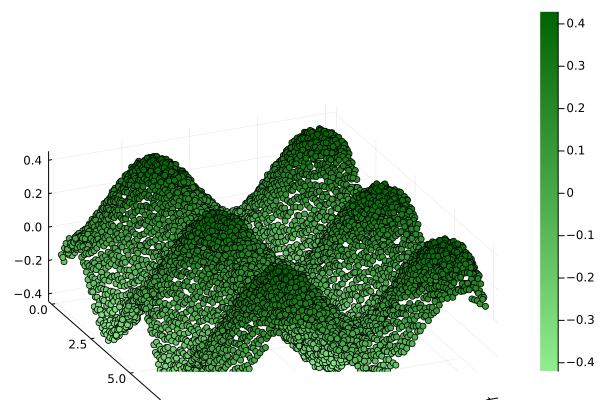
\includegraphics[width=0.7\columnwidth]{graphics/Chap06/WaveFieldData.png}

\vspace*{.2cm}

\begin{lstlisting}[language=Julia,style=mystyle]
using LinearAlgebra

# Function for solving Ax=b using LU decomposition
function solveAxEqb(A,b,aTol=1e-10)
    nRows, nCols = size(A)
    if (length(b) !== nRows)||( nRows !== nCols)
         println("System of equations not properly formed")
        return x=undef
    end
    F=lu(A)
    indicesDiagUsmall=findall(x->x<aTol, abs.(diag(F.U)))
    if length(indicesDiagUsmall) > 0
        println("diagU has numbers that are nearly zero")
        return x=undef
    else
        y=forwardsub(F.L,F.P*b)
        x=backwardsub(F.U, y)
        return x 
    end
end

# Function for fitting data with Least Squares
function LeastSquares_Solve(Phi, Z)
    alpha = solveAxEqb(Phi'*Phi, Phi'*Z) # Phi'*Z = Phi'*Phi * alpha
    Zhat = Phi*alpha
    Error = Z-Zhat
    SqError = Error'*Error
    MeanError = sqrt( SqError/length(Z) )
    return Zhat, Error, SqError, MeanError
end
\end{lstlisting}
\textbf{Output} 
\begin{verbatim}
LeastSquares_Solve (generic function with 1 method)
\end{verbatim}

\begin{lstlisting}[language=Julia,style=mystyle]
# Creating regressor matrix Phi as polynomial fitting
# We include from a constant term, linear terms, quadratic terms, 
# and stop after adding cubic terms
Phi = [ones(Nsq,1) X Y X.^2 Y.^2 X.*Y X.^3 Y.^3 (X).*(Y.^2) (Y).*(X.^2)]
Zhat, Error, SqError, MeanError = LeastSquares_Solve(Phi, Z)
println("Squared error = $SqError and Mean Error = $MeanError")
println("The root mean squared error of our fit is $(MeanError*1e3) mm
    or, if you prefer $(MeanError*1e2/2.54) inches")
\end{lstlisting}
\textbf{Output} 
\begin{verbatim}
Squared error = [260.2866352193259] and Mean Error = [0.16133401229106215]
The root mean squared error of our fit is [161.33401229106215] mm
    or, if you prefer [6.351732767364652] inches
\end{verbatim}


\begin{lstlisting}[language=Julia,style=mystyle]
# Make a scatter plot of Zhat
println("Note how bad the fit is...it does not look like the wavefield at all.")
scatter(X, Y, Zhat, marker_z=Error, legend=false, color = :greens, colorbar=true, camera=(-60, 60))
#png("WaveFieldFit01")
\end{lstlisting}
\textbf{Output} 
\begin{verbatim}
Note how bad the fit is...it does not look like the wavefield at all.
\end{verbatim}

\vspace*{.2cm}

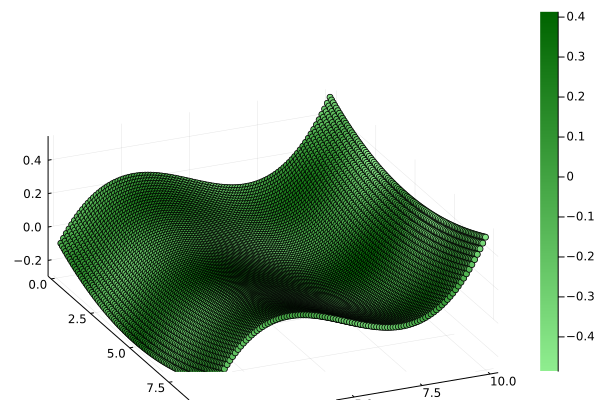
\includegraphics[width=0.7\columnwidth]{graphics/Chap06/WaveFieldFit01.png}


\vspace*{.2cm}

\begin{lstlisting}[language=Julia,style=mystyle]
# Make a scatter plot of the error
println("The fit is so bad, the error looks like the wave field!!!")
scatter(X, Y, Error, marker_z=Error, legend=false, color = :greens, colorbar=true, camera=(-60, 60))
#png("WaveFieldFit01Error")
\end{lstlisting}
\textbf{Output} 
\begin{verbatim}
The fit is so bad, the error looks like the wave field!!!
\end{verbatim}


\vspace*{.2cm}

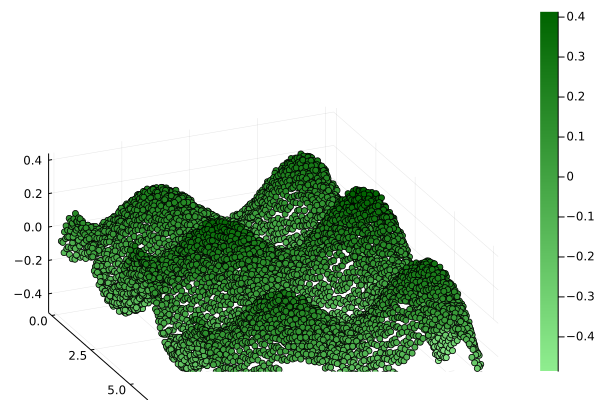
\includegraphics[width=0.7\columnwidth]{graphics/Chap06/WaveFieldFit01Error.png}

\vspace*{.2cm}

\begin{lstlisting}[language=Julia,style=mystyle]
# We'll take another crack at it, using a method that makes it painless to include more terms

# Using for loop to build the regressor matrix Phi
m=8
Phi= Array{Float64,2}(undef, Nsq, 0)
avgX=mean(X)
avgY=mean(Y)
k=0
for i=0:m
    for j=0:m-i
        k=k+1
        Phi=[Phi ((X.-avgX).^i).*((Y.-avgY).^j)/(factorial(i)*factorial(j))]
    end
end
Zhat, Error, SqError, MeanError = LeastSquares_Solve(Phi, Z)
println("Squared error = $SqError and Mean Error = $MeanError")
println("Now see what you think of the fit!")
scatter(X, Y, Zhat, marker_z=Error, legend=false, color = :greens, colorbar=true, camera=(-60, 60))
#png("WaveFieldFit02")
\end{lstlisting}
\textbf{Output} 
\begin{verbatim}
Squared error = [5.066187463106273] and Mean Error = [0.022508192870833218]
Now see what you think of the fit!
\end{verbatim}


\vspace*{.2cm}


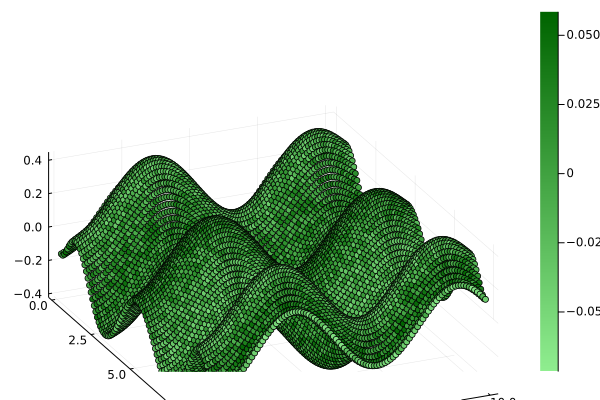
\includegraphics[width=0.7\columnwidth]{graphics/Chap06/WaveFieldFit02.png}


\vspace*{.2cm}

\begin{lstlisting}[language=Julia,style=mystyle]
# Make a scatter plot of the error
println("Now, that's what I call a small error plot.")
scatter(X, Y, Error, marker_z=Error, legend=false, color = :greens, colorbar=true, camera=(-60, 60))
#png("WaveFieldFit02Error")
\end{lstlisting}
\textbf{Output} 
\begin{verbatim}
Now, that's what I call a small error plot.
\end{verbatim}
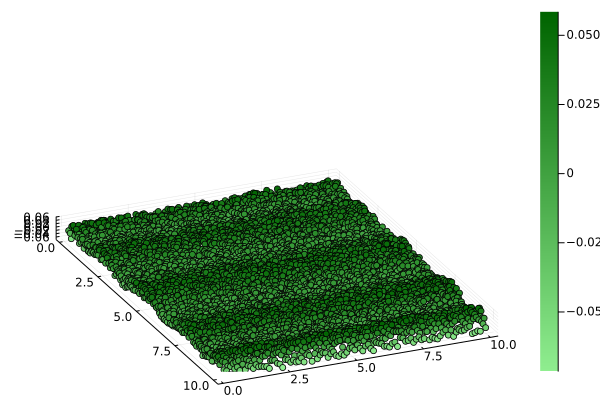
\includegraphics[width=0.7\columnwidth]{graphics/Chap06/WaveFieldFit02Error.png}

\section{(Optional Read) Lab 6.5 A Potpourri of Interesting Commands}

While the tools/commands covered here are not essential for ROB 101, they can make programming either more rewarding or more fun.

\subsection{Using the Benchmark Tool: Which is Faster for Solving Ax=b? }

\begin{lstlisting}[language=Julia,style=mystyle]
using Pkg
Pkg.add("BenchmarkTools")

using LinearAlgebra

function backwardsub(U, b)
    n = length(b)
    x = Vector{Float64}(undef, n) 
    x[n] = b[n]/U[n,n]
    for i in n-1:-1:1
        x[i]=(b[i]- (U[i,(i+1):n])' *x[(i+1):n] )/U[i,i]
    end
    return x
end

function forwardsub(L, b)
    n = length(b)
    x = Vector{Float64}(undef, n) 
    x[1] = b[1]/L[1,1] 
    for i = 2:n 
        x[i]=(b[i]- (L[i,1:i-1])' *x[1:i-1] )/L[i,i] 
    end
    return x
end

function lu_solve(A,b)
    F=lu(A)
    y=forwardsub(F.L,b[F.p])
    x=backwardsub(F.U, y)
    return x
end

function inv_solve(A, b)
    invA = inv(A)
    x = invA*b
    return x
end
\end{lstlisting}
\textbf{Output} 
\begin{verbatim}
inv_solve (generic function with 1 method)
\end{verbatim}

\begin{lstlisting}[language=Julia,style=mystyle]
# We run this cell to compile the functions before using the Benchmark Tool
using Random
Random.seed!(6969420)
N=3
A = rand(N, N)
b = rand(N)
x_inv = inv_solve(A, b)
x_lu = lu_solve(A, b);
\end{lstlisting}
\textbf{Output} 
\begin{verbatim}
Nothing. 
\end{verbatim}

Now, we check the relative speed of the two solvers, using the benchmark tool.
\vspace*{.2cm}
\begin{lstlisting}[language=Julia,style=mystyle]
using BenchmarkTools
Random.seed!(6969420)
N=1000
A = rand(N, N)
b = rand(N)
@benchmark x_inv = inv_solve(A, b)
\end{lstlisting}
\textbf{Output} 

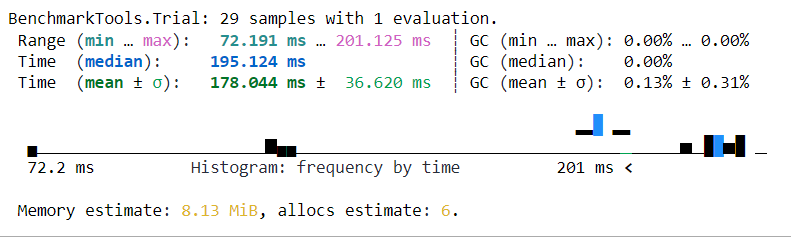
\includegraphics[width=0.7\columnwidth]{graphics/Chap06/BenchmarkInvFunction.png}

\vspace*{.2cm}
\begin{lstlisting}[language=Julia,style=mystyle]
@benchmark x_lu = lu_solve(A, b)
\end{lstlisting}
\textbf{Output} \\

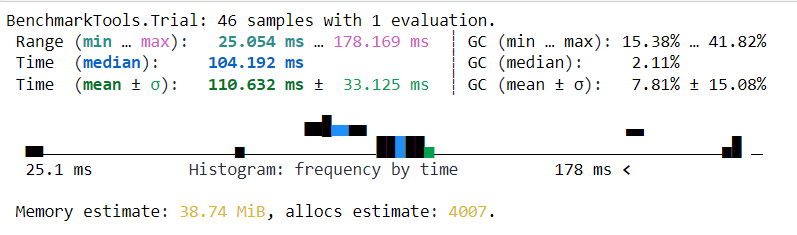
\includegraphics[width=0.7\columnwidth]{graphics/Chap06/BenchmarkLUSolution.png}%

\subsection{Printing with Style and Macros @}


\begin{lstlisting}[language=Julia,style=mystyle]
printstyled("Haha\n", color=:light_cyan)
printstyled("I love ROB 101\n", color=:red, bold=true)
\end{lstlisting}
\textbf{Output} 

\includegraphics[width=0.7\columnwidth]{graphics/Chap06/PrintingWithStyle.png}%


\begin{lstlisting}[language=Julia,style=mystyle]
? printstyled
\end{lstlisting}
\textbf{Output} 
\begin{verbatim}
search: printstyled

printstyled([io], xs...; bold::Bool=false, color::Union{Symbol,Int}=:normal)
Print xs in a color specified as a symbol or integer, optionally in bold.

color may take any of the values :normal, :default, :bold, :black, 
:blink, :blue, :cyan, :green, :hidden, :light_black, 
:light_blue, :light_cyan, :light_green, :light_magenta, 
:light_red, :light_yellow, :magenta, :nothing, :red, :reverse, 
:underline, :white, or :yellow or an integer between 0 and 255 
inclusive. Note that not all terminals support 256 colors. 
If the keyword bold is given as true, the result will be printed in bold.
\end{verbatim}


\begin{lstlisting}[language=Julia,style=mystyle]
macro add_69(num)
    return num+69
end
\end{lstlisting}
\textbf{Output} 
\begin{verbatim}
@add_69 (macro with 1 method)
\end{verbatim}

\begin{lstlisting}[language=Julia,style=mystyle]
@add_69 420
\end{lstlisting}
\textbf{Output} 
\begin{verbatim}
489
\end{verbatim}


\begin{lstlisting}[language=Julia,style=mystyle]
macro add_three_of_them(a, b, c)
    return a+b+c
end
\end{lstlisting}
\textbf{Output} 
\begin{verbatim}
@add_three_of_them (macro with 1 method)
\end{verbatim}

\begin{lstlisting}[language=Julia,style=mystyle]
@add_three_of_them 1 2 3
\end{lstlisting}
\textbf{Output} 
\begin{verbatim}
6
\end{verbatim}

\begin{lstlisting}[language=Julia,style=mystyle]
macro print_in_yellow(x)
    printstyled(x, color=:yellow)
end
\end{lstlisting}
\textbf{Output} 
\begin{verbatim}
@print_in_yellow (macro with 1 method)
\end{verbatim}

\begin{lstlisting}[language=Julia,style=mystyle]
@print_in_yellow "My name is... My name is... My name is... SLIM SHADY"
\end{lstlisting}
\textbf{Output} 


\includegraphics[width=0.7\columnwidth]{graphics/Chap06/PrintInYellow.png}%

\textbf{Julia has an amazing list of Emojis that you can copy and paste into your cells. The symbols will not print in the latex code box below, but they will print in Julia: \url {https://emojidb.org/julia-and-julia-emojis}}

\begin{lstlisting}[language=Julia,style=mystyle]
macro aggressive_print(x)
    s = uppercase(x)
    s*= "!!!!     " # s*= appends the string between the quote marks
                    # The characters do not show here but do work in Julia; see below.
    printstyled(s, color=:red)
end
\end{lstlisting}
\textbf{Output} 
\begin{verbatim}
@aggressive_print (macro with 1 method)
\end{verbatim}


\begin{lstlisting}[language=Julia,style=mystyle]
@aggressive_print "hi nice to meet you"
\end{lstlisting}
\textbf{Output} 



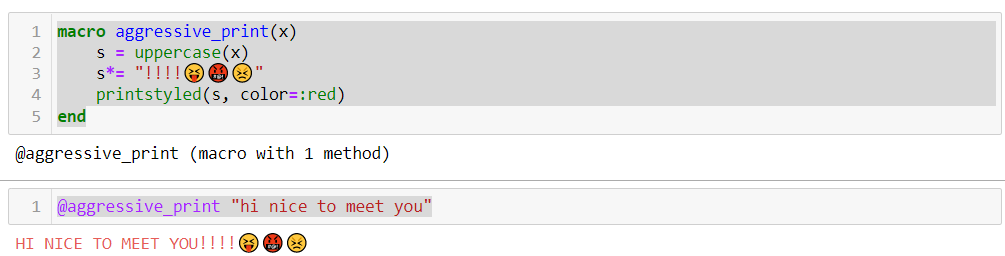
\includegraphics[width=1.0\columnwidth]{graphics/Chap06/AggressivePrint.png}%

\subsection{Multiple Dispatch and Function Overloading}


\begin{lstlisting}[language=Julia,style=mystyle]
function add_them(a::Int, b::Int)
    result = a+b
    return result
end

function add_them(a::Int, b::Vector)
    result = a .+ b
    return result
end

function add_them(a::String, b::Int)
    result = a*string(b)
    return result
end

function add_them(a::String, b::Vector) 
    result = a
    for s in b result*=string(s) end
    return result
end
\end{lstlisting}
\textbf{Output} 
\begin{verbatim}
add_them (generic function with 4 methods)
\end{verbatim}

\begin{lstlisting}[language=Julia,style=mystyle]
@show add_them(2, 3);
@show add_them(2, [3, 4, 5]);
@show add_them("mrbeast", 6000);
@show add_them("gluckgluck", [9,0,0,0]);
\end{lstlisting}
\textbf{Output} 
\begin{verbatim}
add_them(2, 3) = 5
add_them(2, [3, 4, 5]) = [5, 6, 7]
add_them("mrbeast", 6000) = "mrbeast6000"
add_them("gluckgluck", [9, 0, 0, 0]) = "gluckgluck9000"
\end{verbatim}



\begin{lstlisting}[language=Julia,style=mystyle]
import Base:+ 

function +(a::Int, b::Vector)
    result = a .+ b
    return result
end

function +(a::String, b::Int)
    result = a*string(b)
    return result
end

function +(a::String, b::Vector) 
    result = a
    for s in b result*=string(s) end
    return result
end
\end{lstlisting}
\textbf{Output} 
\begin{verbatim}
+ (generic function with 193 methods)
\end{verbatim}

\begin{lstlisting}[language=Julia,style=mystyle]
@show 2 + [3, 4, 5];
@show "mrbeast" + 6000;
@show "gluckgluck" + [9,0,0,0];
\end{lstlisting}
\textbf{Output} 
\begin{verbatim}
2 + [3, 4, 5] = [5, 6, 7]
"mrbeast" + 6000 = "mrbeast6000"
"gluckgluck" + [9, 0, 0, 0] = "gluckgluck9000"
\end{verbatim}
